\chapter{Localization techniques}\label{sec:LocalizationTechniques}
This chapter describes most common techniques and methods for localization. Most of these approaches have multiple implementations and can be also used in parallel to improve accuracy. Fingerprinting for example can be used to increase precision of other methods.

\section{Triangulation}\label{sec:Triangulation}
Methods based on Triangulation use geometric properties of triangles to determine target position. This can be divided further into Lateration and Angulation \cite{RAinWILTaS}. There are multiple sources of data these methods can use, such as distance estimation between device and specific transmitters, measurements of the signal propagation-time (TOA: Time Of Arrival and TDOA: Time Difference of Arrival\cite{LTinWSN}) and the direction of received
signal (AOA: Angle of Arrival\cite{AoALforWSN}) \cite{IILUBLEB}.

\subsection{Lateration}\label{sec:Lateration}
Lateration refers to the technique of determining position based on distance measurements which are calculated using specific devices that know their own position. Mainly used types of Lateration are Trilateration and Multilateration. 

\begin{figure}[h!]
	\begin{centering}
		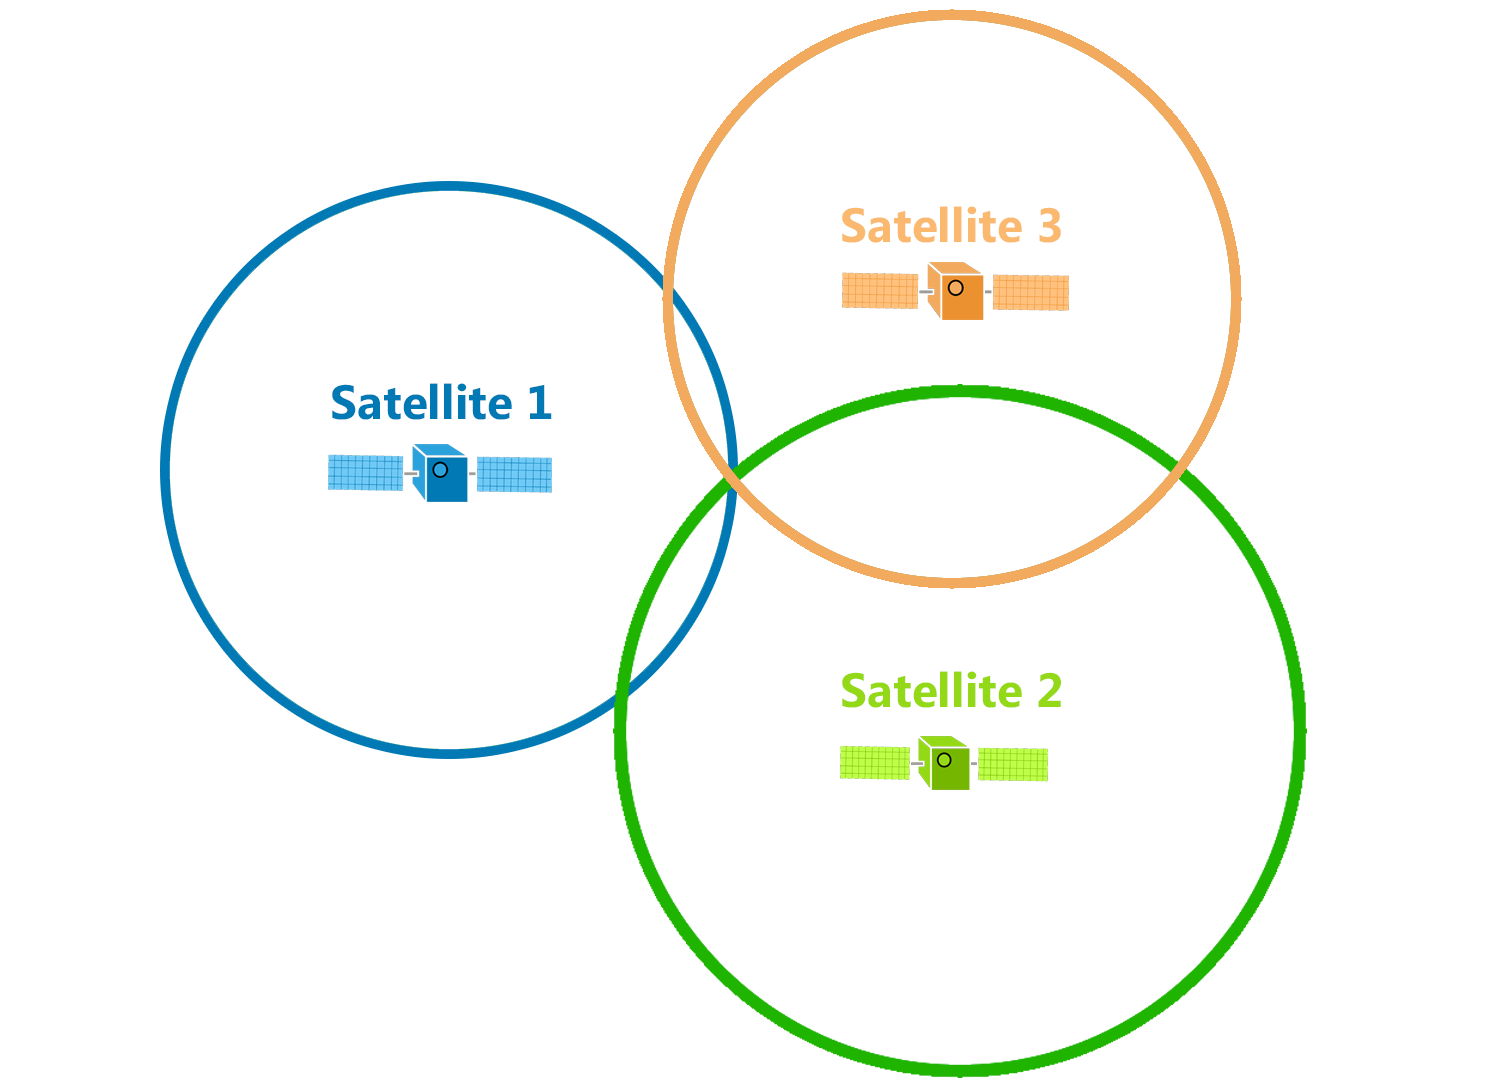
\includegraphics[width=0.48\textwidth]{img/trilateration_2d}
		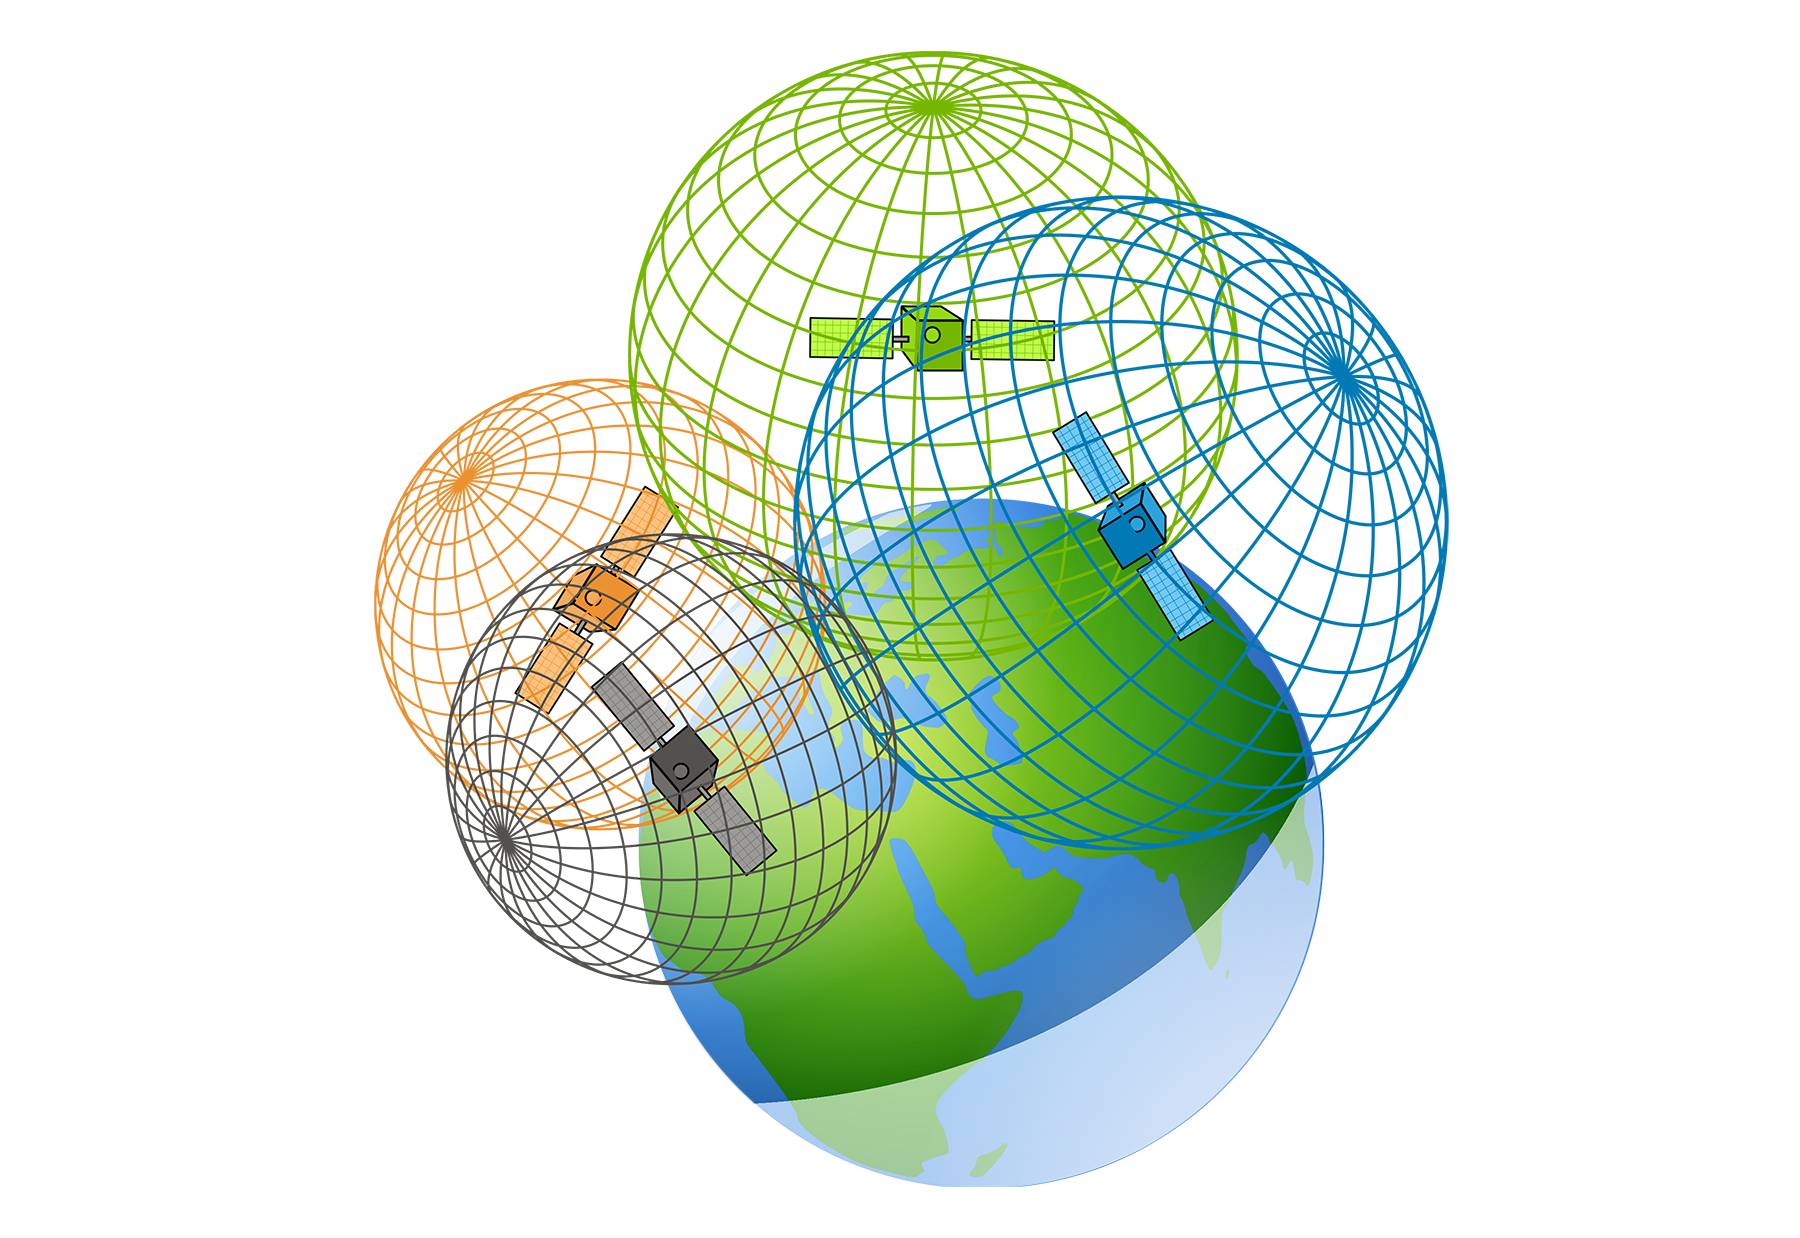
\includegraphics[width=0.48\textwidth]{img/trilateration_3d}
		\par\end{centering}
	\caption{2D and 3D Trilateration (source: \cite{TvTHGPSRW})\label{fig:2d_and_3d_trilateration}}
	\label{fig01c02}
\end{figure}

\textbf{Trilateration} uses distance measurements from at least three devices in particular as \enquote{tri} in the name suggests \cite{RAinWILTaS}. \fref{fig01c02} illustrates usage of Trilateration in 2D and 3D environments. While working in 2D plane will result with only one specific location point, moving to the 3D plane can create a problem because signal is send in a sphere which could result in more than one position. That is the reason why some systems use at least four signal sources to get single location, example of such system is GPS \cite{GNSSGPS}. Advantage of this approach is easy implementation and simple calculations. One downside of this approach is that all devices must have synchronized clock \cite{RAinWILTaS} to prevent localization errors.

\medskip

\textbf{Multilateration}, also known as hyperbolic positioning is using Time Difference of Arrival (TDOA) instead of Time Of Arrival (TOA) used in previous case. This approach uses intersections of hyperbolas rather than circles as shown in \fref{fig02c02}. Main advantage of this method is that only receiving devices must have synchronized clock instead of all \cite{PLTaA}. Multilateration was developed for tracking aircraft position and it is widely used not only for this case.

\begin{figure}[h!]
	\begin{centering}
		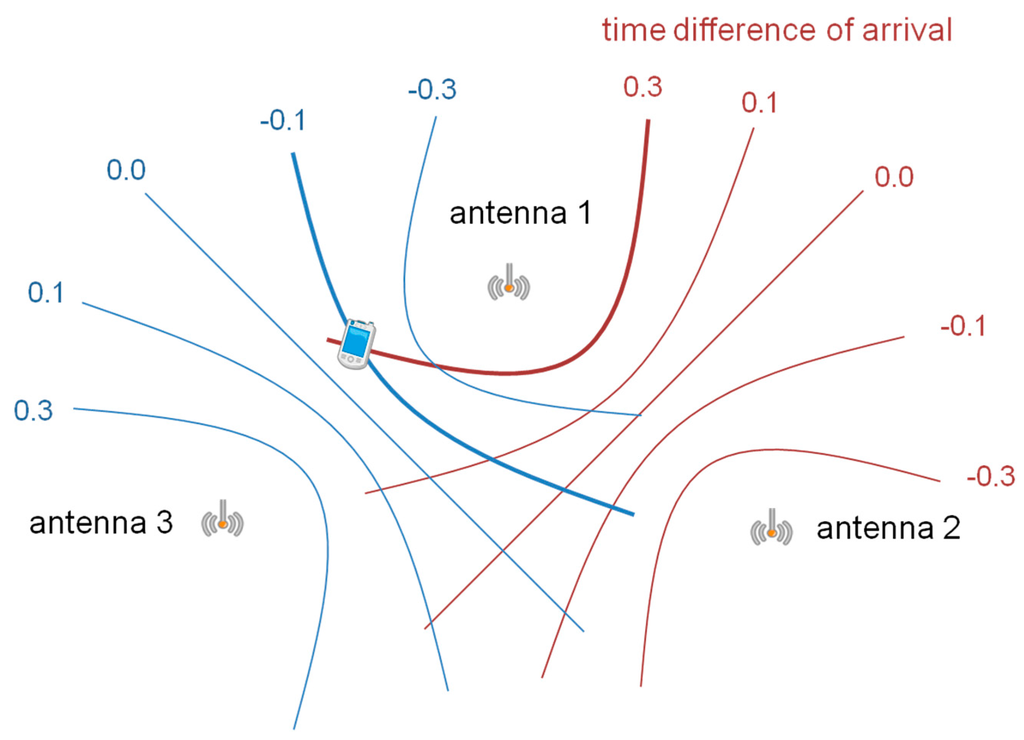
\includegraphics[width=0.6\textwidth]{img/multilateration}
		\par\end{centering}
	\caption{Multilateration (source: \cite{HPwAA})\label{fig:Multilateration}}
	\label{fig02c02}
\end{figure}

Note: At this time term Multilateration is not as strict as it used to be. It can now refer to Lateration with more than three devices.

\subsection{Angulation}\label{sec:Angulation}
This technique uses Angle of Arrival (AOA) of radio signals to determine location and it requires highly directional antennas or antenna arrays. Same as Lateration these antennas are placed in known location and basic AOA requires at least two of them to determine position on 2D plane or more of them to improve accuracy \cite{RAinWILTaS}. Requiring only two antennas is an advantage over Trilateration which requires at least one more. Second advantage of this approach is no need for clock synchronization between devices.

There are also few disadvantages of this approach since it needs complex hardware setup due to the use of directional antennas. Other problem is with multipath locations since it can cause signal reflection and thus making it not useful for indoor localization. And final one to mention is the decrease of accuracy when mobile target moves further from the antennas \cite{AoA, RofAoA}.

\begin{figure}[h!]
	\begin{centering}
		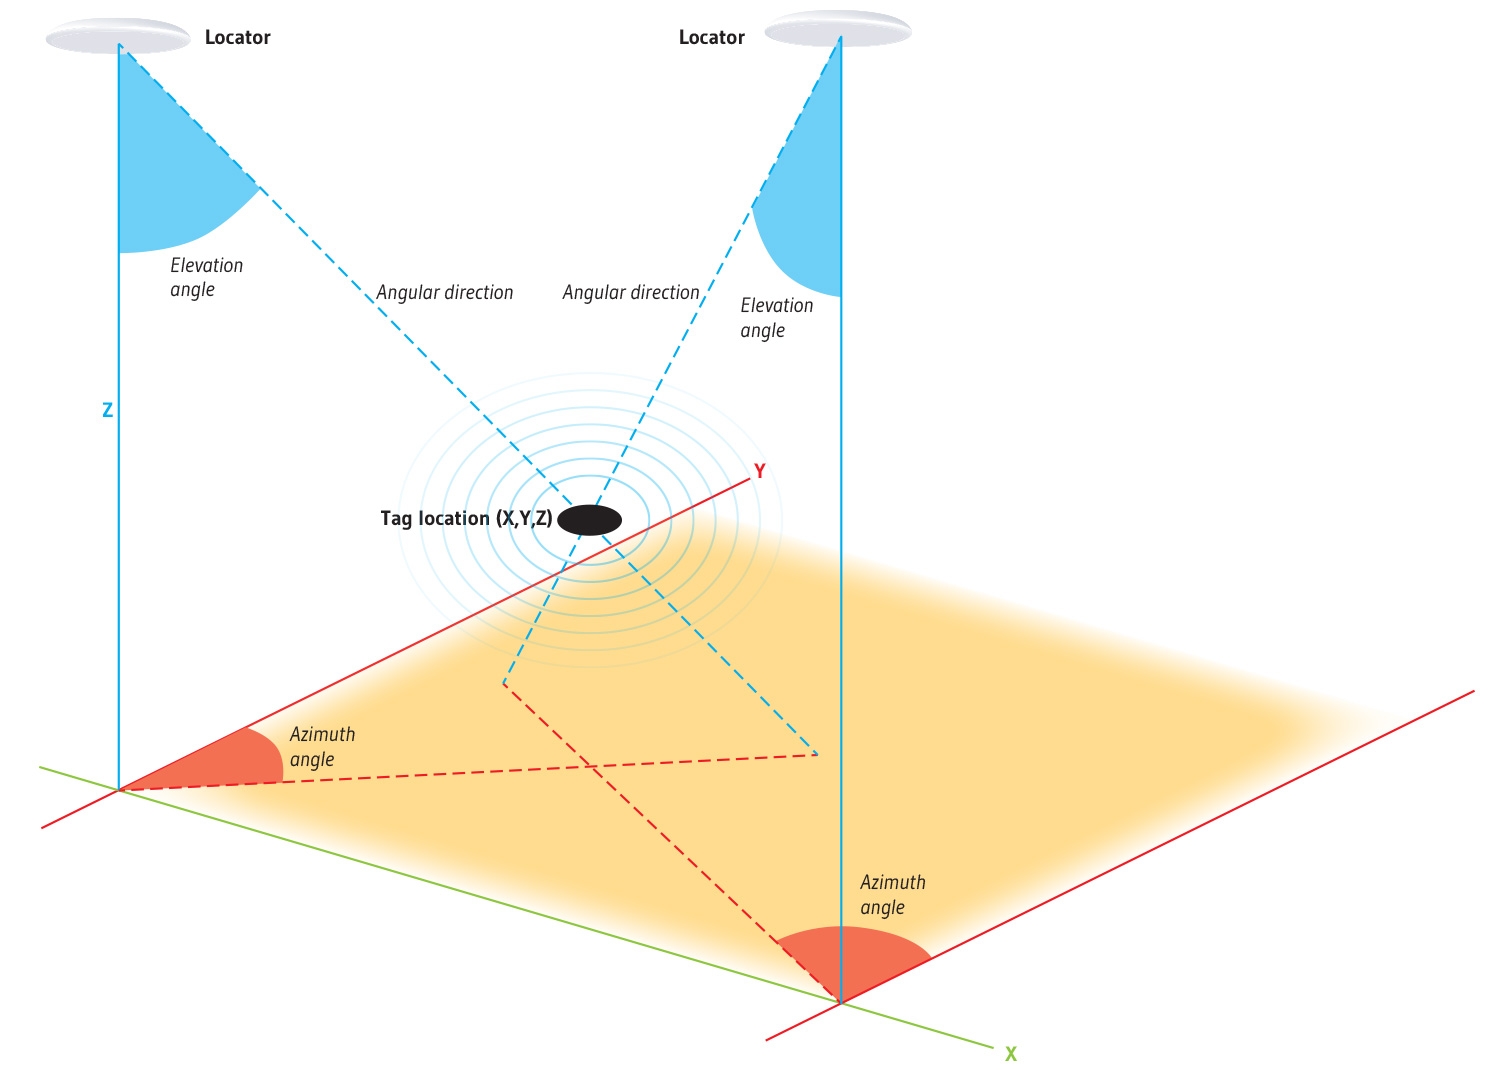
\includegraphics[width=0.6\textwidth]{img/angulation}
		\par\end{centering}
	\caption{3D location using AOA from Quuppa Intelligent Locating System (source: \cite{QAoA})\label{fig:AoAQuuppa}}
	\label{fig03c02}
\end{figure}

\section{Fingerprinting}\label{sec:Fingerprinting}
This method is a part of Signal Strength Fingerprint Maps (SSFM) type. Main point is using previously recorded data in the environment to figure out device location, hence the term fingerprint. There are multiple kinds of radio signal sources, such as bluetooth, wireless or cellular devices that can be recorded.

Fingerprinting is implemented in two main phases. First, fingerprint maps construction also called offline phase. They are created by collecting Received Signal Strength (RSS) and optional extra features in known locations, the specific location is also recorded. All of these values are then saved in the database and that is called fingerprint map. The second phase is localization itself, also known as online phase, where the device measures RSS values and compares them with fingerprint maps to approximate device position using suitable localization method \cite{LocalizationApproaches, ILWTP}. Commonly used algorithms and methods to approximate position are \cite{IILUBLEB}

\begin{itemize}
	\item probabilistic methods,
	\item k-Nearest Neighbors,
	\item neural networks,
	\item support vector machine,
	\item smallest M-vertex polygon.
\end{itemize}

There are multiple advantages of this approach and the most important is that it does not need any additional or specialized hardware. Next one is no need for time synchronization between the devices. Both of these advantages make it simple and cost effective method for localization. On the other hand building of maps is very time consuming and it needs heavy calibration. It is also susceptible to changes in the environment, such as people presence, object movement or relative humidity \cite{IILUBLEB, RSSFofIFD}.

\section{Proximity}\label{sec:Proximity}
Proximity detection, also known as connectivity based positioning, calculates only approximate location. Position is determined by cell of origin (COO) method with known position and limited range \cite{RAinWILTaS}. Device location is based on the cell of connected transmitting device (\enquote{associated access} point in Wi-Fi 802.11 systems) as shown in \fref{fig04c02} \cite{WiFiLBS}.

\begin{figure}[h!]
	\begin{centering}
		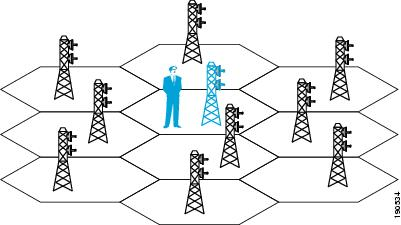
\includegraphics[width=0.6\textwidth]{img/cell_of_origin}
		\par\end{centering}
	\caption{Cell of Origin (source: \cite{WiFiLBS})\label{fig:CellOfOrigin}}
	\label{fig04c02}
\end{figure}

Main advantage of this approach is very easy implementation and no need for complicated algorithms, making calculations really fast. However, for various reasons, devices can be associated to cells that are not in close physical proximity. Such errors can happen for example in multi-floor buildings where floor cells overlap. There are additional methods that can be used to improve this localization, such as using received signal strength indication (RSSI), manual method (human search) or connecting to device with highest signal strength \cite{WiFiLBS, RAinWILTaS}.

\section{Other techniques}
\textbf{Scene analysis} is a pattern recognition method that uses features of the scene observed from a particular vantage point to draw conclusions about the location of observer or objects in the scene \cite{LSfUC}. This approach has been used in many cases, such as image and speech recognition as well as location \cite{LSAWIFI}. The advantage of this technique is that the location of objects can be inferred using passive observation and features. The disadvantage is the need for observer to have access to the features of environment against which they will compare its observed scene \cite{LSfUC}.

\medskip

\textbf{Dead Reckoning} refers to a positioning solution that is implemented by measuring or deducing displacements from a known starting point in accordance with motion of the user \cite{DRNS}. Basically, calculating new position based on starting point, travel distance and angle of movement. New position calculations are dependent on previously calculated ones, creating the need for high accuracy of collected data since it makes errors cumulative \cite{IDRAIP}.